\documentclass{amsart}
\usepackage{amsmath, amssymb, amsthm, hyperref, enumitem, multicol, caption, graphicx, float}

\usepackage[english]{babel}
\usepackage[autostyle, english=american]{csquotes}

\graphicspath{ {images/} }

\setlength{\parskip}{\baselineskip}

\MakeOuterQuote{"}

\newenvironment{Figure}
  {\par\medskip\noindent\minipage{\linewidth}}
  {\endminipage\par\medskip}

\usepackage[margin=1in]{geometry}
\usepackage{listings}
\lstset{
  basicstyle=\ttfamily\scriptsize,
  mathescape
}

\usepackage{fancyhdr}

\title{SKAML: Simulating Known Actors with Machine Learning}
\author{Bryan~Cai, Yasyf~Mohamedali\\ \MakeLowercase{bcai, yasyf}}

\begin{document}

\begin{titlepage}
\centering
~
\vspace{7 cm}
\maketitle
~\\
May 14, 2017
\vfill

\end{titlepage}

\section{Abstract}
\textbf{TODO: ABSTRACT}
Rise of biometric identification \\
downside is hard to change if someone can mimic \\
one metric current systems use is to look at how users type \\
have a existing system from last year, show it is insecure \\
develop models to fool system and simulate how the user types \\
also build new model to distinguish between real user and other users \\
structure of paper \\

\begin{multicols*}{2}
\section{Introduction}

The past few years have seen several attempts to increase security in password-based authentication systems by adding secondary factors derived from biometric patterns in user behavior. Examples of this include Yang and Haddad's \texttt{punchTimeAuth} \footnote{http://css.csail.mit.edu/6.858/2017/projects/yangjy-ddh.pdf} and the commercial product being developed by UnifyID \footnote{https://unify.id}. However, there has not been much focus on the barrier this presents to attackers who are capable of mimicking their targets, particularly in the age of commodity cloud hardware and effective deep learning methods.

We present an exploration into the pitfalls of relying on input-delay-based biometric data as a second factor for authentication, using \texttt{punchTimeAuth} as our standard for comparison. We show that the model introduces a prohibively high number false negatives when exposed to real-world usage. Furthermore, we present serveral adversarial models which can successfully impersonate a user typing their password, trained on background typing data that need not include the password itself. In order to collect this data, we built two collection mediums: a Google Documents look-alike and an extension for Google Chrome. We collect which keys are pressed, the length of time each is held for, and the delay between each pair of keys. Finally, we present a novel neural model for attempting to distinguish users based on the information we collect, along with some conclusions and observations about this source of data as a second factor for security.

All of the code for this paper can be found at \url{https://github.com/yasyf/skaml}.

\section{Threat Model}

Our exploration focuses specifically on the systems which analyze the delays between a user's keypresses while she is typing her password. We assume that the system in question has been previously trained with multiple samples of the user's typing patterns. Our tests were against the seventh quantile-based \texttt{punchTimeAuth}. We assume the role of an adversary which has managed to obtain the password of a user (such as through a database breach, phishing scam, or cross-site scripting exploit), and is attempting to gain access to a system employing the second factor of security described above. We further assume that the adversary has time to build tools as we did to collect typing data on their target. Importantly, we do not require the adversary to ever witness their target typing the password in question.

\section{Approach}
\subsection{Data Collection}

In order to collect sufficient typing data from the users that agreed to participate in our exploration, we built two interactive tools. In both cases, we solicited complacent users by inviting them to use our applications, relying on their lack of careful inspection when receiving a link from someone they trust.

The first is a Google Docs look-alike \footnote{https://snarl.herokuapp.com}, which imitates a well-known service in a phishing-style attempt to convince a complacent user to type on the page. We overlayed a text box on a webpage containing the CSS from a Google Doc we created, allowing the user to type as if this were the application they are so familiar with. We implemented a small client-side library in JavaScript which listens for the \texttt{KeyDown} and \texttt{KeyUp} DOM events emitted from the textbox, so as to record the length of time each key is held for and the delay between key presses, as well as the actual characters being typed. This data is stored in a local buffer and is periodically uploaded to our servers, where a a Flask app records the logged objects to a MongoDB instance, tagged with a unique identifier for the user in question.

\begin{figure}[H]
  \centering
  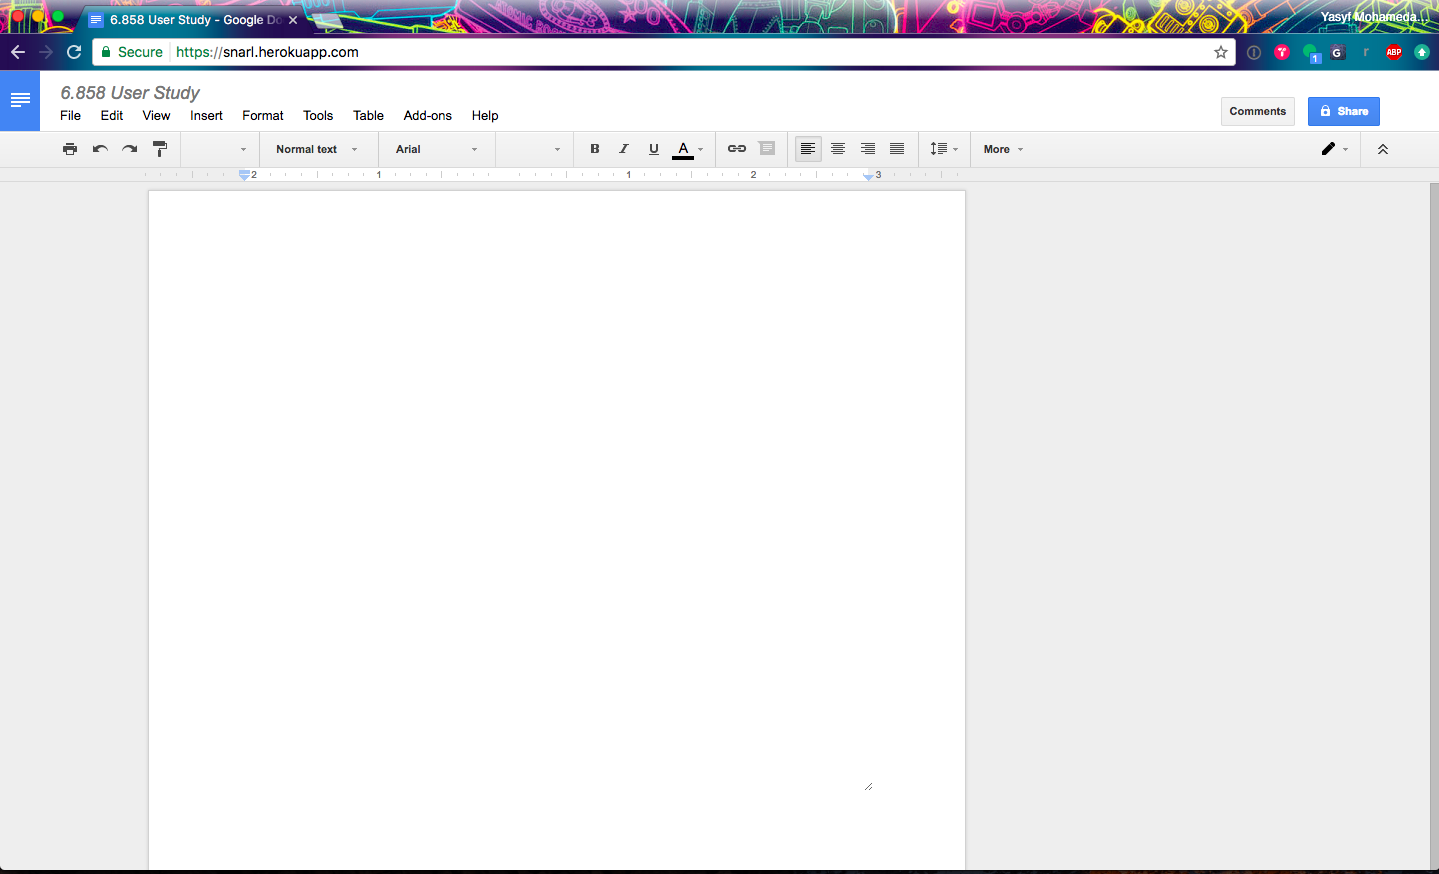
\includegraphics[width=0.4\textwidth]{gdocs}
  \caption{Google Docs look-alike}
\end{figure}

The second technique we developed for data collection is a key-logging Google Chrome extension \footnote{https://snarl.herokuapp.com/client}. While the data quality from a document editor was vastly superior to the flow of data from casual bursts of typing in a browser, our models demanded as much data as we could possibly collect. Thus we augmented our corpus by creating an extension that injects a script into every web page, using the same library as before. We asked participants to install the extension and made them aware of the implications; our proof-of-concept was installed with consent but could just as easily be installed through less transparent means by a bad actor.

The combined results of these two methods resulted in a data set of approximately $25000$ character pairs across several users.

\subsection{Models}
\subsubsection{Means Model}
For this project we trained several types of models. We first focused on the problem of tricking a security system into believing that we, as a hypothetical bad actor, were the original user, by simulating the delays that the original user would have in their password typing.

To begin, we trained a simple means model to estimate the delay a specific user exhibits between any two characters, regardless of context. We simply used the average delay between a given pair of characters for the user in question, filling in missing data with a global mean. This model performed surprisingly well.

\subsubsection{Neural Models}
Our first neural model has the goal of mimicking how a user types, building on the simple means model and capturing additional context. For each use when given a sequence of letters, the model outputs a sequence of delays between each consecutive pair of letters that mimics how the user would have typed those letters. It does this one pair at a time; the model takes as input $W$ letters preceding and $W$ letters following the pair we are predicting. For each of these $N$ letters, the model constructs a vector of length $V$, which represents the forward and backwards context in the word. Using these two vectors, one delay is produced. Iterating over every consecutive pair of letters gives the desired sequence of delays.

The next model, the distinguisher, tries to achieve the opposite effect; given a sequence of letters and timings, it tries to guess whether the sequence was typed by the user. This model takes as input a sequence of vectors, where each vector encodes what letter was typed, how long the key was held down for, and the delay from the last keypress.

\section{Implementation}

We built a Python backend in Flask with an API to support our collection and processing. This included routines to receive JavaScript objects with \texttt{KeyCode}s and translate them to one-hot vectors which could be fed into our neural models. In order to aid with supervision of the collection process, we built several tools and dashboards to explore the data being collected.

\begin{figure}[H]
  \centering
  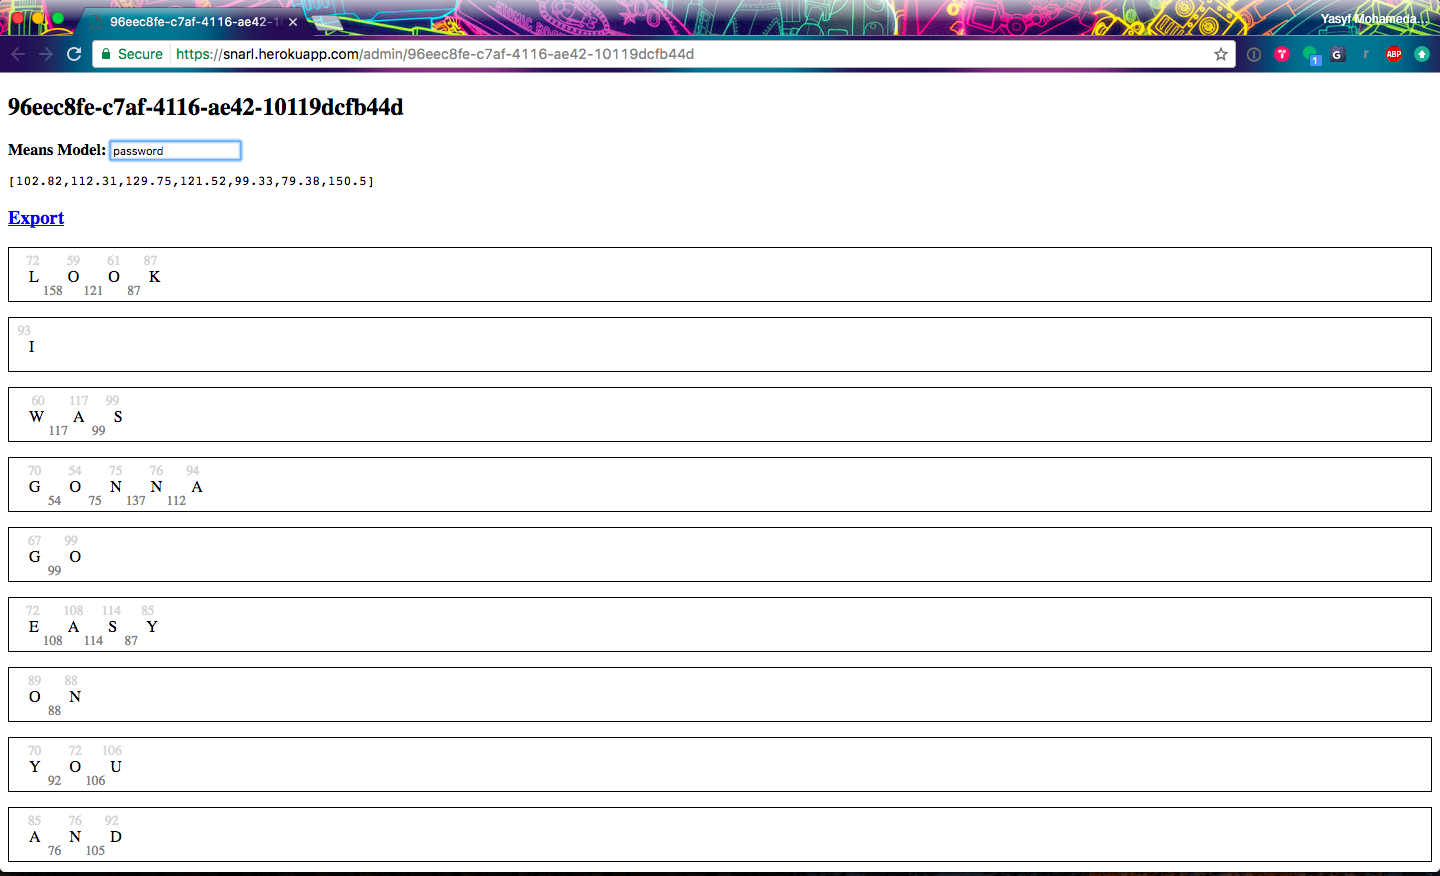
\includegraphics[width=0.4\textwidth]{admin}
  \caption{Data Debgging Dashboard}
\end{figure}

\subsection{Models}
\subsubsection{Means Model}
Our means model for a given user $u$ was the result of a few simple NumPy operations, with the final \texttt{means} matrix defined as follows. \texttt{means} is an $N \times N$ matrix, where $N = |\mathcal{C}|$ is the cardinality of the set of characters that can appear in a string. For simplicity, we limited this set to lowercase letters, numbers, and punctuation. Element $(i, j)$ of \texttt{means} indicates the predicted user delay between typing character $i$ and character $j$.

Let $y_u$ be the flattened length-$n$ vector of measurements $(c_1, c_2, \texttt{delay})$ taken for user $u$, where $\texttt{delay}$ is the delay between this particular instance of typing $c_1$ and $c_2$. Let $N_{c_1, c_2} = \texttt{count}(y_u : c_1 = i, c_2 = j)$.

\[ \texttt{means}[i][j] :=
  \begin{cases}
      \frac{\sum_{y_u : c_1 = i, c_2 = j}{\texttt{delay}}}{N_{c_1, c_2}} & N_{c_1, c_2} > 0 \\
      \frac{\sum_{\texttt{means} : N_{i, j} > 0}{\texttt{means}[i][j]}}{\texttt{count}(\texttt{means} : N_{i, j} > 0)} & N_{c_1, c_2} = 0 \\
   \end{cases}
\]

\subsubsection{Neural Models}
The neural models were implemented in Python, using Keras with a TensorFlow backend. Characters were represented using one-hot vectors, and delays and hold times were measured in milliseconds. We first discuss the mimic model. This model takes two $W \times A$ matrices, where $W$ is the size of the context we consider and $A$ is the alphabet size. The first matrix represents the forward context, and the second matrix represents the backwards context. For example, if the word is "SECURITY," if we had a window size of 4 and we are trying to predict the delay between the "R" and the "I", the first matrix is the sequence of one-hot vectors representing ["C", "U", "R", "I"] and the second is the sequence of one-hot vectors representing ["R", "I", "T", "Y"]. If there are not enough letters, we pad the matrix with zero vectors. Each of these $W \times A$ matrices is fed through an RNN that produces the intermediate vector of length $V$. We then concatenate these two vectors and feed it through a fully connected layer with 50 nodes, and then then to a final output node. We used the mean absolute error as the loss function, and standard gradient descent as the optimizer.

The distinguisher model takes as input a matrix of size $L \times (A + 2)$, where $L$ is the maximum word length we allow, which is set to 15 but can be set higher in the future if necessary. Each row of the matrix consists of the one-hot vector of length $A$, with the keydown time and delay time appended. This is fed through one RNN layer, then through several dense layers, culminating in an final layer with 2 outputs and softmax activation.

\section{Results}
\subsection{Means Model}

As we will discuss later, the laborious and manual process of training systems like \texttt{punchTimeAuth} left us in the difficult position of not having many options for automated testing. Thus, our testing efforts were the result of us randomly sampling words and attempting to have our model type them in the fashion of the training user. The same user would train the security system by using that word as their password for a new account, and we would inject JavaScript to simulate our predicted delays at a login screen. Using this method, our means model was able to successfully imitate several users 90\% of the time. This result is somewhat surprising, given that we did not expect users to necessarily type in a document editor the same way they type a familiar password.

\subsection{Neural Models}

\textbf{TODO: RESULTS}

\section{Discussion}

We faced serval challenges in collecting data and implementing the models for this exploration. One of the largest barriers to rigorous results was the fact that the systems we attempted to break all require significant effort to train. Concretely, in order to evaluate an imitation of a user's typing of a specific password, that user must train the security system on how she types that password. This high barrier to the end user is a shortcoming of the string-specific model used in \texttt{punchTimeAuth}, and something we tried to address with our generalized neural distinguisher. However, as we discovered, simple typing timing and language context do not provide sufficient information to produce a generalized model of a user's biometric profile.

Another particularly interesting challenge occured in the client-side data collection library we authored. Detecting lengths of key presses in addition to delays meant we could not simply listen for \texttt{KeyPress} events, and put us at the mercy of the JavaScript event loop scheduler. We spent nontrivial amount of time post-processing the stream of events we received to piece together the sequence of user key presses.

On the data collection front, we experienced expected challenges including a lack of willing study participants, and foreign scripts interfering with our injected collection routines in the browser.

\textbf{TODO: KEYBOARD DISTANCE THING}

\section{Conclusion}

\textbf{TODO: CONCLUSION}

\textbf{TODO: CITATIONS}

\end{multicols*}
\end{document}

\grid
